% ============================================================================
% Paper C — Dissecting Online Learning Mechanisms:
%   Statistical Memory, Homeostatic Recovery, and Substrate Physics
%   are Non-Transferable
% ============================================================================
% Compiles standalone: pdflatex PAPER_C.tex (run twice for cross-refs).
% Figures resolve via ../figures/ (extension-less basenames).
% ============================================================================
\documentclass[10pt,twocolumn]{article}

\usepackage[margin=1in]{geometry}
\usepackage{amsmath,amssymb}
\usepackage{booktabs}
\usepackage{graphicx}
\graphicspath{{../figures/}}
\usepackage{microtype}
\usepackage[hidelinks]{hyperref}
\usepackage{url}

\title{Dissecting Online Learning Mechanisms: Statistical Memory,
Homeostatic Recovery, and Substrate Physics are Non-Transferable}
\author{[Author Name]\\[2pt] Independent Researcher, Guiyang, China\\
\small\texttt{[author@example.com]}}
\date{}

\begin{document}

\maketitle

\begin{abstract}
Online learning systems couple several adaptive mechanisms, but which
mechanism is responsible for which capability --- and whether any of them
can be transplanted to another substrate --- is rarely tested. We dissect
three mechanisms of a reservoir-based online learner: a slow-trace
statistical memory (M3), a homeostatic chaos regulator (M5), and the raw
physics of the substrate itself. A falsifying transfer experiment
(ESN with and without the metadata under a sequential disturbance chain,
10 seeds) shows that the previously reported $+32\%$ sequential-recovery
gain is produced by the homeostat, not by the metadata, and that the
metadata does not transfer memory-capacity robustness to an ESN at any
metadata timescale ($\tau_m \in \{200,500,1000,2000\}$, paired differences
$-0.68$ to $-0.70$, 0/10 seeds positive). The metadata's transferable
value is narrower and precisely located: it denoises \emph{state}-level
corruption (gap $-0.69 \rightarrow -0.01$ when noise enters before the slow
trace) and accelerates boundary adaptation by a controlled-measured factor
of 1.3--2.4 on the substrate and $\sim$10 pulses on the ESN (the published
``$9$--$20\times$'' ratios were window-position metric artifacts). Raw
memory capacity remains a substrate property (MC 10.19 vs.\ 6.17). Three
mechanisms, three roles --- and none is transferable to another's job.
\end{abstract}

\section{Introduction}
\label{sec:intro}

Frozen batch models --- including large foundation models --- cannot adapt
to post-deployment reality without expensive retraining; online reservoirs
can, but their readouts face a timescale gap on long-horizon statistical
tasks: fast reservoir states decorrelate far more quickly than the task
statistics, so the readout must re-integrate after every change. Recent
work on our side adds a slow exponential trace of the reservoir states
(metadata, M3), a homeostatic regulator that keeps the substrate near the
edge of chaos (M5), and slow structure plasticity (M4); the integrated
system tracks drift where frozen learners fail permanently
(companion Paper~B).

These mechanisms are usually validated \emph{together}. The question we
ask here is sharper: \emph{which mechanism does which job, and can any of
them be transplanted to another substrate?} We answer with a deliberately
falsifying experiment: take a generic echo-state network (ESN), give it
the same metadata, run it through the same sequential disturbance chain,
and measure what transfers. The answer is largely negative and,
we argue, informative: the metadata is a substrate-agnostic
\emph{statistical} memory that transfers \emph{accuracy} and
\emph{state-noise denoising}, but not \emph{memory-capacity robustness}
under readout-level disturbance; sequential recovery is the homeostat's
job; raw memory capacity is the substrate's physics. Three mechanisms,
three roles --- none substitutable.

\section{Setup}
\label{sec:setup}

\textbf{Reservoir family.} We compare (i)~an ESN-256 with heterogeneous
leak rates matched to a log-normal spectrum ($\mathrm{CV}=0.20$, spectral
radius 0.9) and (ii)~a Si$_3$N$_4$-style relaxation substrate whose
per-unit time constants are log-normal (median $\tau_0\approx174\,\mu$s,
$\mathrm{CV}=0.20$), driven in per-pulse contrast-coupled dynamics with
coupling $\kappa$ (companion Paper~A). Both produce a fast state
$x(t)\in\mathbb{R}^{256}$ per pulse.

\textbf{Slow trace (M3).} The metadata is a per-unit exponential moving
average
\begin{equation}
m(t) = \left(1-\frac{1}{\tau_m}\right) m(t-1)
     + \frac{1}{\tau_m}\, x(t),
\label{eq:ema}
\end{equation}
with algorithmic timescale $\tau_m$ (pulses), and the readout feature is
$\varphi(t) = [x(t),\, m(t),\, 1]$.
\label{eq:feat}

\textbf{Readout.} OnlineRLS with forgetting $\lambda_f=0.999$ (weight
integration time $\tau_f = 1/(1-\lambda_f)=1000$ pulses),
predict-before-update, Tikhonov-regularized.

\textbf{Tasks and metrics.} \emph{regime\_switch}: 3 regimes with
overlapping pulse-interval distributions, regime changes every
$L=1500$ pulses; single pulses are almost indistinguishable across regimes
--- only long-run statistics discriminate. \emph{Mackey--Glass online
prediction} under a sequential disturbance chain. Metrics: overall
accuracy, switch-relative adaptation time $T_{\mathrm{adapt}}$ (pulses
after a \emph{known} switch to reach a 200- or 40-pulse window accuracy of
0.98/0.95), and the Jaeger held-out memory capacity (MC) probe.

\textbf{Sequential disturbance chain (substrate-agnostic).} Three
cumulative disturbances at $t=7$k/14k/21k pulses: (1)~timescale drift
(substrate $\tau \times 1.5$; ESN leaking rate $/1.5$), (2)~structure
prune (40\% of connections), (3)~readout noise ($\sigma=0.1$ on the
features). Per-round MC is probed at the settled physics.

\section{Theory: the slow trace is a synthesized forgetting kernel}
\label{sec:theory}

\textbf{Proposition 1 (kernel synthesis).} The input-to-slow-trace channel
implements a forgetting kernel with a zero at zero lag, a finite peak lag,
and an exponential tail whose $1/e$ horizon is exactly $\tau_m$ --- an
externally controllable, substrate-independent parameter. If the fast
state has kernel $h_x$, the slow channel kernel is the convolution of the
EMA impulse response with $h_x$; for $h_x(u)=e^{-u/\tau_x}$,
\begin{equation}
h_m(\Delta t)
= \frac{e^{-\Delta t/\tau_m} - e^{-\Delta t/\tau_x}}{\tau_m - \tau_x},
\qquad h_m(0)=0,\quad \mathrm{peak}\sim
\frac{\tau_m\tau_x}{\tau_m-\tau_x}\ln\frac{\tau_m}{\tau_x}.
\label{eq:kernel}
\end{equation}
The material kernel of Paper~A, $M(\Delta t)=\int p(\tau)\,e^{-\Delta
t/\tau}\,d\tau$ (log-normal), is fixed by physics; $h_m$ is synthesized
by the algorithm, and the augmented system's effective kernel is
$M \circledast h_m$ with $1/e$ horizon $\sim \tau_m + \tau_0$ (Fig.~\ref{fig:kernel}).

\textbf{Proposition 2 (timescale coverage).} On the statistical task the
bottleneck is missing slow modes, not substrate physics. Both fast channels
decorrelate at $\tau_{\mathrm{eff}} \ll L$; the slow trace supplies the
missing timescale to either substrate, so accuracy and adaptation converge
to a common band. Measured (S10, 10 seeds): esn-fast 0.9955, esn-dual
0.9979, REDEM 0.9942; steady accuracy 1.000 for all.

\textbf{Proposition 3 (feature stationarity).} Post-switch adaptation is
bounded by the slower of feature re-centering ($\sim \tau_m + \tau_{\rm
eff}$) and weight re-integration ($\sim \tau_f$). The slow trace makes
recovery feature-limited rather than weight-limited. Under a controlled
switch-relative protocol (S15/S5b), the true effect is modest but real: on
the substrate the fast readout needs $T_{200}=265$--$304$ pulses to
re-stabilize vs.\ $202$--$211$ for dual (factor 1.3--1.4 on $T_{200}$,
1.6--2.4 on $T_{40}$); on the ESN, $T_{40}$ drops from 49.9 to 40.6 with
the p90 collapsing from 76.5 to 42.0. The published ``$9$--$20\times$''
ratios were ratios of window positions with near-zero denominators
(metric artifacts), not pulse times.

\textbf{Proposition 4 (noise geometry).} The EMA is a first-order low-pass
filter, $|H(\omega)|^2 = 1/(1+(\omega\tau_m)^2)$. Short fast-channel
transients are attenuated in the metadata channel. The transferable value
of this is \emph{denoising of state-level corruption}: when the noise
enters the states before the slow trace is computed, the metadata nearly
neutralizes it (S16b variant V2). It does \emph{not} protect against
readout-level noise that hits the metadata channel equally (variant V0).

\section{Experiments}
\label{sec:exp}

\subsection{Equalization on the statistical task (S10)}
\label{sec:s10}

Table~\ref{tab:s10} reproduces the equalization result: the same slow
trace ($\tau_m=500$) closes the accuracy gap between the ESN and the
substrate and collapses adaptation variance. All arms sit in the
$[0.994,\,0.998]$ band with steady accuracy 1.000.

\begin{table}[t]
\centering
\small
\begin{tabular}{lccc}
\toprule
arm & overall acc & steady acc & $T_{40}$ (pulses) \\
\midrule
esn-fast & $0.9955\pm0.0015$ & 1.000 & $49.9$ ($p_{90}=76.5$) \\
esn-dual ($\tau_m{=}500$) & $0.9979\pm0.0001$ & 1.000 & $40.6$ ($p_{90}=42.0$) \\
REDEM (substrate, dual) & $0.9942\pm0.0011$ & 1.000 & $52.7$ ($p_{90}=67.0$) \\
\bottomrule
\end{tabular}
\caption{S10 equalization on regime\_switch (10 seeds). Accuracy from
\texttt{data/s10\_esn\_metadata\_v1.*}; adaptation from the controlled
S15 protocol (\texttt{data/s15\_controlled\_adaptation\_v1.*}).}
\label{tab:s10}
\end{table}

\subsection{The falsifying transfer experiment (S14)}
\label{sec:s14}

Under the sequential disturbance chain, the substrate regulated by the
homeostat (M5) recovers: $r_3$ MC $8.47\pm0.39$ vs.\ $6.41\pm0.41$ for the
fixed arm ($+32\%$), with $\kappa$ drifting $25.3\rightarrow28.5$
(Table~\ref{tab:s14}; S11 protocol, features are fast-state only --- the
recovery is purely homeostatic). The ESN with the same metadata does
\emph{not} recover: paired per-seed differences
$r_3\,\mathrm{MC}(\text{esn-dual}) - r_3\,\mathrm{MC}(\text{esn-fast})$ are
$-0.78$/$-0.76$/$-0.69$ at $r_1$/$r_2$/$r_3$, with 0/10 seeds positive in
every round ($\sim$5$\times$ the paired std). The $+32\%$ sequential
recovery therefore belongs to the homeostat, not the metadata.

\begin{table}[t]
\centering
\small
\begin{tabular}{lccccc}
\toprule
arm & $r_0$ MC & $r_1$ MC & $r_2$ MC & $r_3$ MC & $r_3$ NMSE \\
\midrule
esn-fast & 6.17 & 1.82 & 1.76 & 1.74 & 0.0277 \\
esn-dual & 6.16 & 1.04 & 1.00 & 1.05 & \textbf{0.0251} \\
redem-reg & \textbf{10.19} & 7.17 & 7.51 & \textbf{8.47} & 0.1063 \\
\bottomrule
\end{tabular}
\caption{S14 disturbance chain (10 seeds; \texttt{data/s14\_esn\_disturbance\_chain\_v1.*}).
redem-reg reproduces the S11 anchor exactly (10.19/7.17/7.51/8.47).}
\label{tab:s14}
\end{table}

\subsection{Pressure test across metadata timescales (S16)}
\label{sec:s16}

Does any $\tau_m$ let the metadata close the MC gap? No: at
$\tau_m\in\{200,500,1000,2000\}$, the dual arm's $r_3$ MC is
1.04/1.05/1.06/1.06 vs.\ 1.74 for fast, with paired differences
$-0.701$/$-0.693$/$-0.682$/$-0.678$ and 0/10 seeds positive at every
timescale (Table~\ref{tab:s16}, Fig.~\ref{fig:recovery}left). There is no
sensitive interval; the weak upward trend (1.04$\rightarrow$1.06) does not
approach the baseline. Meanwhile the readout-noise attenuation transfers
at every $\tau_m$ ($r_3$ NMSE 0.0235--0.0254 vs.\ 0.0277;
Fig.~\ref{fig:recovery}right).

\begin{table}[t]
\centering
\small
\begin{tabular}{lcccc}
\toprule
$\tau_m$ & dual $r_3$ MC & fast $r_3$ MC & paired diff & $n_{\mathrm{pos}}$ \\
\midrule
200 & 1.04 & 1.74 & $-0.701$ & 0/10 \\
500 & 1.05 & 1.74 & $-0.693$ & 0/10 \\
1000 & 1.06 & 1.74 & $-0.682$ & 0/10 \\
2000 & 1.06 & 1.74 & $-0.678$ & 0/10 \\
\bottomrule
\end{tabular}
\caption{S16 tau\_m pressure test (10 seeds;
\texttt{data/s16\_tau\_m\_pressure\_test\_v1.*}).}
\label{tab:s16}
\end{table}

\subsection{Probe-protocol stress test (S16b)}
\label{sec:s16b}

The falsification is robust \emph{in sign} to the probe protocol: under
standardized slow features (V1) and state-level noise injection (V2),
every ($\tau_m$, variant) cell keeps 0/10 seeds positive
(Table~\ref{tab:s16b}). Its \emph{magnitude} is protocol-dependent and
informative: under readout-noise semantics (V0, the S11/S14 definition)
the gap is $-0.69$; under state-noise semantics (V2) the metadata's EMA
denoising nearly closes it ($-0.01$). This locates the metadata's
transferable value precisely: it denoises \emph{state}-level corruption,
not readout-level noise.

\begin{table}[t]
\centering
\small
\begin{tabular}{lccc}
\toprule
variant & dual $r_3$ MC & paired diff & $n_{\mathrm{pos}}$ \\
\midrule
V0 readout noise & 1.05/1.06 & $-0.69/-0.68$ & 0/10 \\
V1 std-slow & 1.08/1.07 & $-0.66$ & 0/10 \\
V2 state noise & 1.72/1.73 & $-0.015/-0.009$ & 0/10 \\
\bottomrule
\end{tabular}
\caption{S16b probe-protocol stress test ($\tau_m=500/2000$; 10 seeds;
\texttt{data/s16b\_falsification\_stress\_test\_v1.*}). Fast baseline
$r_3$ MC 1.74.}
\label{tab:s16b}
\end{table}

\subsection{Controlled adaptation (S15/S5b)}
\label{sec:s15}

With known switch instants, the honest adaptation advantage of the
metadata is a factor 1.3--2.4 on the substrate (T200: fast 264.8--303.9
vs.\ dual/slow 202--211 pulses) and $\sim$10 pulses on the ESN
($T_{40}$ 49.9$\rightarrow$40.6, p90 76.5$\rightarrow$42.0), with overall
accuracy reproducing S5/S10 exactly. The published ``$9$--$20\times$''
ratios were window-position metric artifacts.

\section{Discussion}
\label{sec:disc}

\textbf{Three mechanisms, three roles.} The evidence assembles a clean
decomposition. (i)~\emph{Metadata (M3) = statistical memory}: it supplies
the missing timescale on statistical tasks (S10), denoises state-level
corruption (S16b V2), and attenuates readout noise on the online task
(S14/S16 NMSE) --- but it adds no episodic memory capacity (r0 MC
unchanged) and cannot recover memory under readout-level disturbance at
any $\tau_m$ (S14/S16/S16b). (ii)~\emph{Homeostat (M5) = disturbance
recovery}: the $+32\%$ sequential recovery (S11) and $+18\%$ $r_1\!\to\!r_3$
(S14) are produced by $\kappa$-regulation alone; the metadata is not
involved. (iii)~\emph{Substrate physics = raw memory}: the MC probe puts
the substrate at 10.19 vs.\ $\sim$6.17 for either ESN arm; no algorithm in
this work closes that lead.

\textbf{Why non-transferability is informative.} Each mechanism has a
precisely located job, and swapping them fails in a measurable way. This
delineates the boundary conditions of ``metadata transfer'' claims in the
online-reservoir literature: transfer holds for accuracy and
state-noise denoising, and does not hold for disturbance recovery or
episodic memory.

\textbf{Related work.} The slow trace is the linear slow-feature operator
on reservoir states (cf.\ slow feature analysis, Wiskott \& Sejnowski
2002); the fast/slow pair is a two-timescale memory hierarchy echoing
complementary learning systems \cite{mcclelland1995} and synaptic
consolidation \cite{benna2016}; the readout computes a fading-memory
functional \cite{boyd1985} whose horizon the metadata extends without
touching the substrate.

\textbf{Limitations.} The slow trace's attenuation covers fast-channel
(readout or state) corruption; direct corruption of the metadata memory
itself is out of scope. $\tau_m$ remains a hyperparameter tuned to the
task timescale. The substrate's homeostat requires a Lyapunov estimate
(FTLE) that we do not provide for the ESN.

\textbf{Future work.} Consolidating stable, repeatedly encountered
knowledge into the structural connectivity would create a hierarchy
between fast tracking and slow accumulation, but introduces a
consolidation-vs-overwrite trade-off beyond the present scope.

\section{Conclusion}
\label{sec:concl}

(1)~A slow exponential trace of reservoir states is a synthesized
forgetting kernel with a controllable horizon (Prop.~1). (2)~On
long-horizon statistical tasks the bottleneck is timescale coverage, not
substrate physics; the same trace equalizes ESN and substrate accuracy and
accelerates adaptation by a controlled-measured factor 1.3--2.4 (Props.~2--3).
(3)~The trace is a \emph{statistical} memory, not an episodic one: it adds
no raw memory capacity and does not transfer disturbance robustness at any
$\tau_m$ (0/10 seeds positive; Prop.~4, S14/S16/S16b). (4)~Three
mechanisms, three roles --- metadata (statistical memory and state-noise
denoising), homeostat (sequential recovery), substrate physics (raw
memory) --- and none is substitutable for another's job.

\section*{Code and data availability}
All simulation scripts and generated data are available at
\url{https://github.com/huyamingc/REDEM} (private during review; released
on acceptance). Paper C data: \texttt{data/s10\_esn\_metadata\_v1.*},
\texttt{data/s11\_disturbance\_chain\_v1.*},
\texttt{data/s14\_esn\_disturbance\_chain\_v1.*},
\texttt{data/s16\_tau\_m\_pressure\_test\_v1.*},
\texttt{data/s16b\_falsification\_stress\_test\_v1.*},
\texttt{data/s15\_controlled\_adaptation\_v1.*},
\texttt{data/s5b\_controlled\_adaptation\_v1.*}.

\begin{figure}[t]
\centering
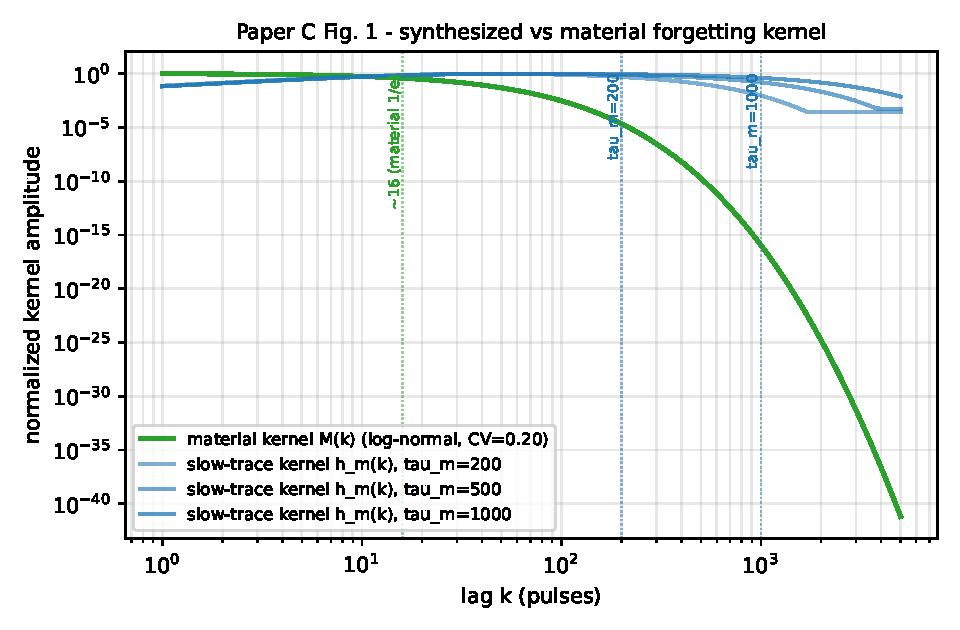
\includegraphics[width=0.9\columnwidth]{paperC_fig1_kernel}
\caption{Synthesized vs.\ material forgetting kernel (Paper C, Fig.~1):
the slow-trace kernel $h_m$ (Eq.~\ref{eq:kernel}, $\tau_m =
200/500/1000$ pulses) has a zero at zero lag, a finite peak lag, and an
exponential tail with $1/e$ horizon exactly $\tau_m$; the material kernel
$M$ (Paper~A, log-normal, CV 0.20) is fixed by physics (1/e $\sim$16
pulses).}
\label{fig:kernel}
\end{figure}

\begin{figure}[t]
\centering
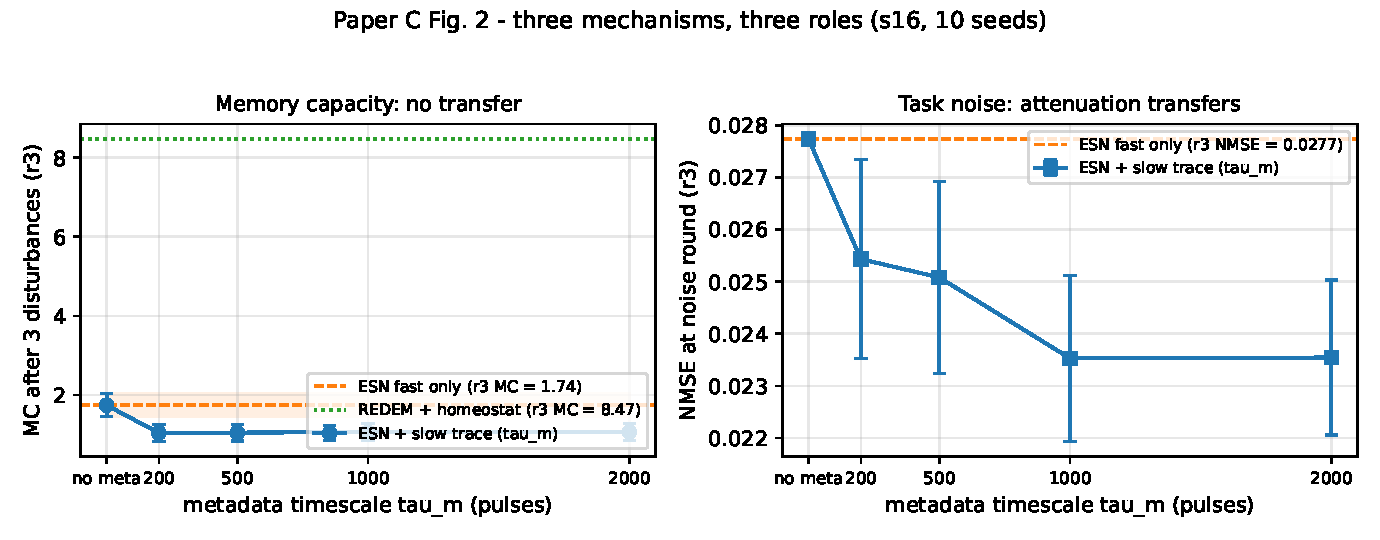
\includegraphics[width=0.9\columnwidth]{paperC_fig2_recovery}
\caption{Post-disturbance recovery vs.\ metadata timescale (Paper C,
Fig.~2; s16, 10 seeds). Left: $r_3$ MC --- esn-dual stays 0.68--0.70
below esn-fast at every $\tau_m$, while the homeostat-regulated substrate
(redem-reg, no metadata) sits at 8.47. Right: $r_3$ NMSE --- the
readout-noise attenuation transfers at every $\tau_m$.}
\label{fig:recovery}
\end{figure}

\begin{thebibliography}{11}

\bibitem{jaeger2001} Jaeger, H. The ``echo state'' approach to analysing
and training recurrent neural networks. GMD Report 148 (2001).

\bibitem{maass2002} Maass, W., Natschläger, T., Markram, H. Real-time
computing without stable states. \emph{Neural Computation} \textbf{14}(11),
2531--2560 (2002).

\bibitem{boyd1985} Boyd, S., Chua, L. O. Fading memory and the problem of
approximating nonlinear operators with Volterra series. \emph{IEEE
Transactions on Circuits and Systems} \textbf{32}(11), 1150--1161 (1985).

\bibitem{mcclelland1995} McClelland, J. L., McNaughton, B. L., O'Reilly,
R. C. Why there are complementary learning systems in the hippocampus and
neocortex. \emph{Psychological Review} \textbf{102}(3), 419--457 (1995).

\bibitem{benna2016} Benna, M. K., Fusi, S. Computational principles of
synaptic memory consolidation. \emph{Nature Neuroscience} \textbf{19}(12),
1697--1706 (2016).

\bibitem{wiskott2002} Wiskott, L., Sejnowski, T. J. Slow feature analysis:
unsupervised learning of invariances. \emph{Neural Computation}
\textbf{14}(4), 715--770 (2002).

\bibitem{companionA} Author's companion Paper A: Memory and chaos in a
physics-constrained relaxation substrate: phase diagram, multi-timescale
forgetting, and disturbance robustness (substrate theory; target:
\emph{International Journal of Bifurcation and Chaos} / \emph{Chaos}).

\bibitem{companionB} Author's companion Paper B: REDEM: Training-Inference
Unified Learning with Meta-Adaptation and Structural Plasticity for
Non-Stationary Environments (online learning architecture; target:
\emph{Neural Networks}).

\end{thebibliography}

\end{document}
